\documentclass[12pt]{article}

\usepackage{tema2014}

\usepackage{graphicx,url}

%\usepackage[brazil]{babel}
\usepackage[utf8]{inputenc}


\sloppy

\title{Modelo de documento para as conferências da TeMA}

\author{Marcos da Silva Sampaio\inst{1}}

\address{Grupo de Pesquisa Genos ---
         Escola de Música da Universidade Federal da Bahia \\
         Av. Araújo Pinho, 58 ---
         40110-913 Salvador, BA
         \email{marcos@sampaio.me}
}

\begin{document}

\maketitle

\begin{abstract}
  Versão traduzida do resumo.
\end{abstract}

\begin{resumo}
  Este meta-arquivo descreve o estilo a ser usado na elaboração de
  artigos para submissão nas conferências da Associação Brasileira de
  Teoria e Análise Musical (TeMA). O resumo deverá conter uma
  introdução, o objetivo do projeto trabalhado, a metodologia, os
  resultados (parciais ou finais) e apontar as conclusões. O resumo
  deverá ter, no máximo de 250 palavras, sem parágrafo e sem citações
  bibliográficas.
\end{resumo}


\section{Introdução}
\label{sec:gen}

Este modelo inclui toda a informação referente à formatação de artigos
para as conferências da TeMA. Este guia deve ser seguido para que os
anais dos eventos tenham um padrão uniforme. Este modelo pode ser
obtido na página da TeMA (http://tema.mus.br).


\section{Tamanho da página}
\label{sec:tamanho-pagina}

Os anais serão organizados em formato A4 retrato (21.0cm x 29.7cm).
Todo o conteúdo de cada página deve caber dentro do retângulo de
17.2cm x 25.2cm, centralizado na página, com margens 2cm (topo), 2.5cm
(base), 2cm (esquerda/direita). O texto deve estar inteiramente
justificado, com separação de sílabas.

\section{Fonte}
\label{sec:fonte}

Todo o texto deverá ter fonte Times. Fontes sem serifa e não
proporcional só podem ser usadas com propósitos especiais, como para
diferenciar texto de código-fonte de programas.

\section{Primeira página}

A primeira página deve conter o título do artigo, o nome e endereço
dos autores, o abstract em inglês e o resumo em português (nos textos
em português). O título deve ser centralizado sobre a página, com
fonte Times em negrito 16pt.

Os nomes dos autores devem estar centralizados, com fonte Times 12pt,
em negrito, todos dispostos em uma mesma linha, separados por
vírgulas. Os endereços devem estar centralizados, com fonte Times
12pt. O abstract deve ter fonte Times itálico 12pt, em itálico, indentado em 0.8cm
em ambos os lados.


\section{Título e autores}

A fonte do título é Times, 14pt, negrito, caixa alta e centralizada.
Os nomes dos autores são omitidos na submissão para revisão. Para a
versão final, os nomes dos autores deverão estar centralizados. O nome
do autor principal deverá ser o primeiro e o dos co-autores depois,
separados por vírgulas. Se os endereços dos autores for o mesmo, este
deve ser inserido apenas uma vez, centralizado. Se os endereços forem
diferentes, deverão ser espaçados, sob os nomes dos autores.


\section{Seções e parágrafos}

Os títulos de seções devem ter fonte Times, negrito, 13pt, e
alinhamento à esquerda. Deve haver um espaço extra de 12 pt antes de
cada título. A numeração das seções é obrigratória. O primeiro
parágrafo de cada seção não deve estar indentado. Os seguintes devem
ter indentação 0.5cm.

\subsection{Subseções}

Os títulos de subseções devem ter fonte Times, negrito, 13pt, e
alinhamento à esquerda.

% TODO: Copiado do ISMIR. confirmar se irei manter
% \subsection{Informação sobre Copyright}

% A informação de copyright deve ser incluída exatamente como aparece
% aqui, no canto inferior esquerdo da página, em fonte Times 8pt.

\subsection{Números de página, cabeçalhos e rodapés}

O texto não deve conter cabeçalhos, rodapés ou números de página em sua submissão.
Estes elementos serão adicionados quando os anais forem
confeccionados.

% TODO: Seguir com os demais itens

\section{CD-ROMs and Printed Proceedings}

In some conferences, the papers are published on CD-ROM while only the
abstract is published in the Proceedings. In this case, authors are
invited to prepare two final versions of the paper. One, complete, to
be distributed in CD and the other, containing only the first page,
with abstract and ``resumo'' (for papers in Portuguese) for the
printed version.

\section{Figures and Captions}

Figures and tables captions should be centered if less than one line
(Figure~\ref{fig:exampleFig}), otherwise justified and indented by
0.8cm on both margins. The font must be Helvetica, 10 point, boldface,
with 6 points of space before and after each caption.

In tables, do not use colored or shaded backgrounds, and avoid thick,
doubled, or unnecessary framing lines. When reporting empirical data,
do not use more decimal digits than warranted by their precision and
reproducibility.


\begin{figure}
\centering
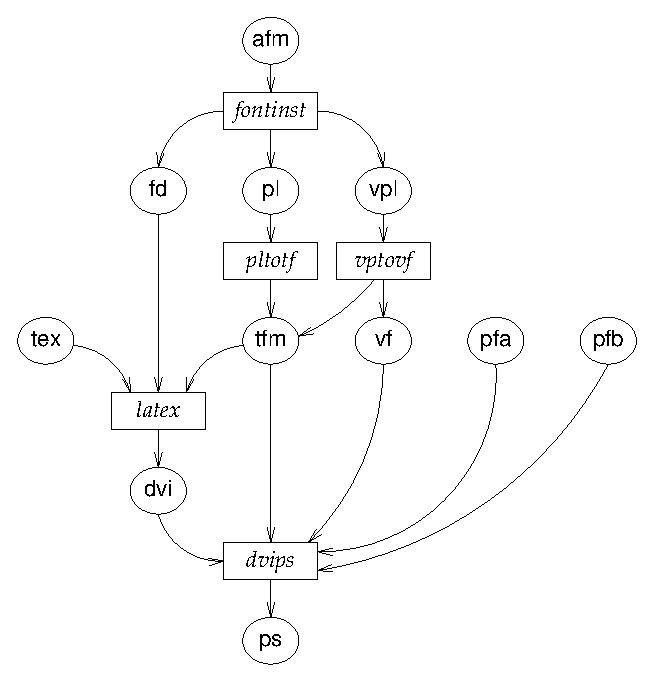
\includegraphics[width=.5\textwidth]{exampleFig.eps}
\caption{A typical figure}
\label{fig:exampleFig}
\end{figure}


\section{Images}

All images and illustrations should be in black-and-white, or gray
tones. The image resolution on paper should be about 600 dpi for
black-and-white images, and 150--200 dpi for grayscale images. Do not
include images with excessive resolution, as they may take hours to
print, without any visible difference in the result.

\section{References}

Bibliographic references must be unambiguous and uniform. We recommend
giving the author names references in brackets, e.g. \cite{knuth:89}, \cite{smith:99}.

\bibliographystyle{apalike}
\bibliography{example}

\end{document}
